
\chapter{Méthode proposée}

L'objectif de notre méthode est d'avoir une reconnaissance multi-vues d'un ou plusieurs objets à la fois, capable d'intégrer le déplacement du robot pour résoudre des ambiguïtés et faux positifs. Pour incorporer les notions de vues et de transition entre elles, on utilise une représentation simple et suffisamment générale basée sur les graphes d'aspect. Le déplacement d'un état à un autre dans ce graphe est ensuite estimé par rapport au déplacement du robot. Ce système est ensuite couplé avec un dispositif de reconnaissance mono-vue classique capable de retrouver la vue la plus probable d'un objet à partir de descripteurs 3D. Une méthode de suivi des objets et un traitement probabiliste de changement de vue étant donné l'information motrice permet enfin d'augmenter le taux de reconnaissance.

\section{Architecture générale}
L'approche a été développée pour une base mobile différentielle munie de capteurs proprioceptifs odométiques et d'une caméra RGB-D. Les informations provenant des ces unités sont envoyés à une unité de traitement qui interprète les images reçues, isole les objets qu'elles contiennent et compare cette interprétation avec une base de données stockée dans la mémoire. En cas d'absence de correspondant dans la base, ce nouvel exemplaire pourra éventuellement être ajouté à la base de données et agrandir les connaissances d'objets existants dans l'environnement.

L'architecture du système est illustrée à la figure \ref{fig:architecture} et permet à la fois, de comprendre les dépendances entre les étapes de traitement, de même que, la nature du flux d'information entre modules.

\begin{figure}[H]
  \centering
  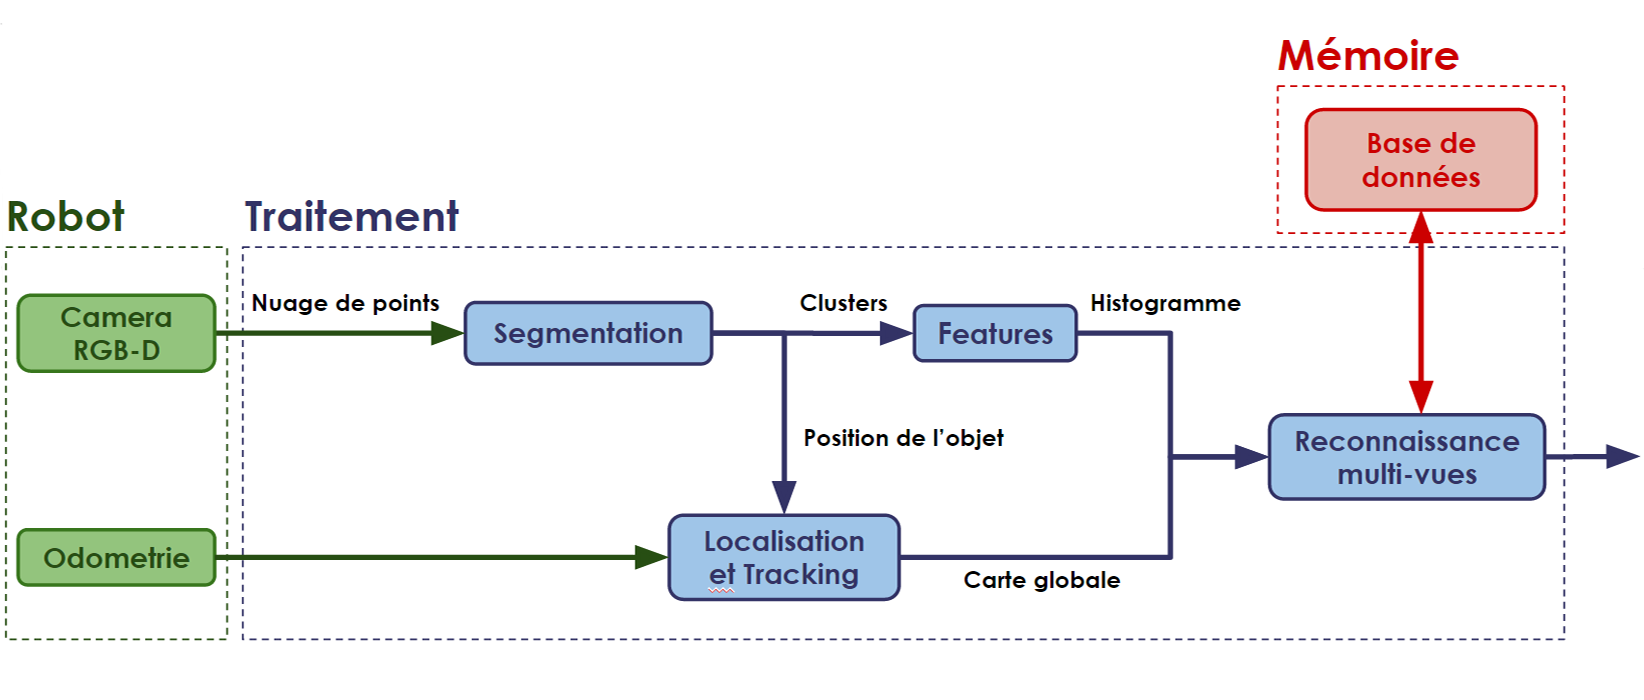
\includegraphics[width=0.95\textwidth]{gen_arc.png}
  \caption{Architecture générale du système}
  \label{fig:architecture}
\end{figure}

Plus précisément, l'unité de traitement reçoit un nuage de points brut provenant de la caméra, ainsi que la mesure de rotation de roues du robot. La première partie du traitement vise à nettoyer le nuage en segmentant des points des objets candidats de la scène, ce qui permet d'enlever une partie non pertinente et de créer un nuage de point dédié pour chaque objet de l'image. Ces nuages de points sont envoyés à l'unité d'extraction de features pour générer des histogrammes représentatif de chaque objets dans l'image. Simultanément, une conversion de référentiel localise des objets dans le repère absolu de déplacement du robot. Puis, les positions des objets sont données au module de localisation et tracking qui suit les observations et les associes entre elles pour avoir une cohérence globale des positions. En dernier lieu, pour chaque objet, les histogrammes de features ainsi que leurs positions converties dans un repère global sont envoyées au module de reconnaissance, et sont utilisés pour reconnaitre les éléments de la scène et donner leur vue la plus probable à chaque instant de temps. 

Les prochaines sections détaillent l'architecture présentée à l'image \ref{fig:architecture}, en présentant le fond théorique derrière le fonctionnement de chaque sous-module.

\section{Segmentation}

La segmentation consiste à isoler des objets dans une image brute, ou en d'autres termes, différencier les éléments qui ne constituent pas un objet et les objets eux-mêmes. La segmentation d'objets est considérée comme un élément essentiel en traitement d'image étant donné qu'une fois l'objet séparé du fond, la reconnaissance devient beaucoup plus simple. La difficulté majeure d'un tel algorithme sur des images RGB vient du fait que la projection de la scène sur le plan image supprime l'information de profondeur. Les capteurs stéréoscopiques et infra-rouges permettent de compenser cette absence d'information et simplifient énormément le traitement nécessaire.

Dans le cas où le capteur est immobile, on utilise classiquement des méthodes de soustraction de fond pour l'étape de segmentation \cite{dai2006prospects}. Ceci n'est pas possible dans notre cas car le robot évolue dans son environnement. La démarche proposée par la littérature dans ce cas considère les objets comme des ensembles de points délimités par un seuil de proximité. Cette définition est suffisamment générale pour permettre de représenter une grande quantité d'objets. Néanmoins, définir ces ensembles dans une image brute n'est pas forcément simple. Par conséquent, on utilise un nouvel \textit{a priori} qui spécifie que les objets se situent sur des plans de support. Bien que plus restrictif que la définition d'avant, cela permet un segmentation crédible. Parmis les méthodes de segmentation se basant sur cette définition, on peut citer Tabletop object detector \cite{tabletop} qui détermine le plan principal de l'image (généralement une table ou le sol) grâce à l'algorithme RANSAC \cite{fischler1981random}, puis recherche des objets dans l'enveloppe convexe de ce plan. Par ailleurs, Caron et al. \cite{caron2014neural} ont proposé une approche légèrement différente. En partant du même principe, le sol est estimé, puis un traitement pour le fond de la scène est appliqué, où les plans orthogonaux à la normale du sol et de taille suffisamment grands sont considérés comme des murs, et les éléments trop près des bords ne sont pas considérés. 

\subsection{Algorithme}

La méthode de segmentation utilisée dans notre cas est celle proposée par Caron et al. Cette méthode s'applique surtout pour de la segmentation d'objets posés sur le sol dans des environnements intérieurs et répond aux exigences du domaine de déplacement du robot : le laboratoire de Thales Theresis.\\

Plus spécifiquement, elle peut être découpée selon les étapes suivantes :
\begin{enumerate}[start=0]
\item Calibration permettant d'obtenir l'équation du sol avant le début de la séquence.
\item Soustraction du sol à partir de l'équation trouvée
\item Filtrage des points trop éloignés, considérés comme plus incertains
\item Calcul de la normale des surfaces de la scène
\item Élimination de murs, considérés comme des grands plans orthogonaux au sol
\item Voxelisation des points non filtrés pour accélérer le traitement
\item Projection des points voxelisés dans le plan du so
\item Regroupement des points en objets grâce à l'algorithme de \textit{clustering} point growing de PCL
\item Calcul du centroïde et des bounding boxes 2D et 3D de chaque objet
\end{enumerate}

Ainsi, l'algorithme fournit la position de chaque objet dans le repère de la caméra ainsi que le nuage de point et les normales qui leur sont associés.

Une calibration initiale est nécessaire pour définir l'équation du sol. Pour cela, on place le robot dans un endroit où l'image obtenue correspond majoritairement au sol. L’équation du plan dominant est extrait par RANSAC et sauvegardée dans un fichier texte. %Une explication plus détaillée sur les sous-méthodes utilisées pour chaque étape est présentée dans les annexes, ainsi qu'une discussion sur les paramètres utilisés.


\subsection{Restrictions} 
La physique des capteurs restreint le type d'objets qui peuvent être aperçus et segmentés, soit à cause des réflexions des rayons infra-rouges, soit à cause de la
résolution limitée des images mesurées. D'un autre côté, la segmentation a ses propres contraintes en ce qui concerne le positionnement des objets dans l'image et, principalement, la définition du sol et des murs. Par conséquent, les restrictions de l'algorithme sont les suivantes :

\begin{itemize}
\item Le sol où le robot se déplace n'est pas accidenté.
\item L'objet se trouve par terre à une distance inférieure à 3 mètres .
\item La lumière ambiante ne doit pas contenir trop de lumière infra-rouge.
\item L'objet n'est ni transparent ni trop réflectif et dépasse le seuil d'appartenance au sol.
\end{itemize} 

Un grand nombre d'objets, entre autres chaises, tables, écrans, boîtes en carton, poubelles, de tailles et formes variés ont été testés et peuvent être segmentés malgré les restrictions. Une exemple de segmentation est présenté dans la figure \ref{fig:mono_recon} pour illustrer la capacité de segmentation. 

\section{Descripteurs}


Le travail des descripteurs est, d'une part, d'extraire des caractéristiques intéressants de l'élément observé et, d'autre part, de réduire la
dimensionnalité de l'espace traité, tout en restant robuste à des transformations affines et aux changements de luminosité. On s'intéresse surtout ici aux descripteurs basés sur le nuage de point des objets, bien qu'il soit possible aussi d'utiliser des descripteurs associés à la texture ou à la couleur. Les descripteurs qui nous intéressent sont des descripteurs géométriques qui essaient de traduire les idées de courbure, de forme et taille dans les histogrammes, et sont intéressants pour étudier les ambiguïtés de reconnaissance. Parmis les descripteurs 3D proposés dans la littérature, on peut citer FPFH \cite{rusu2009fast} qui est invariant par changement de point de vue, SHOT \cite{tombari2010unique} étant un descripteur local de courbure et des descripteurs semi-globales orientés au traitement des occlusions CVFH \cite{aldoma2011cad} et Our-CVFH \cite{aldoma2012our}. Une description détaillée de ces descripteurs et leurs principales différences sont expliquées dans les annexes \ref{annexe:descripteur}. Nous choisissons d'utiliser le descripteur \textit{Viewpoint Feature Histogram} - VFH, car il permet de discriminer non seulement les formes géométriques (pour la reconnaissance d'objet), mais aussi les points de vues (reconnaissance de vue).

En partant de l'hypothèse que la segmentation propose un découpage correct des objets, on extrait des descripteurs globaux à partir des ensembles de points proposés. Ainsi, pour chaque objet, on obtient un histogramme VFH représentatif de l'objet et de la vue segmentée.

\section {Reconnaissance mono-vue} 
\label{sec:rec_mono}

Afin de reconnaitre les objets et leur points de vue rencontrés par le robot, nous utilisons les histogrammes de descripteurs VHF et une base de donnée réalisée à l'avance. Dans cette base, les histogrammes de plusieurs objets sont calculés pour plusieurs points de vues ainsi que leurs positions relatives (Plus de détails sur la construction de la base à la section \ref{sec:base_donnees}). Le but est de retrouver l'objet et son point de vue le plus proche par rapport à la base. Pour cela, il est possible d'utiliser des algorithmes de \textit{machine learning} classiques, mais les résultats sur des réseaux de neurones n'ont pas été très concluants. Aldoma et al. \cite{Aldoma2012} suggèrent l'utilisation de la mesure de similarité entre histogrammes chi-squared, associée au classificateur \textit{k plus proches voisins}, ou K-NN. Le gros avantage de ce classificateur est l'étape d’apprentissage, qui correspond à création d’un arbre de recherche construit à partir de la comparaison croisée entre les éléments de la base. Par rapport aux données dont nous disposons, cet arbre se construit et fournit une estimation du plus proche voisin de manière presque instantannée.

L'API de la librairie FLANN sur PCL permet l'utilisation directe du classificateur K-NN. L'implé- mentation permet l'utilisation de plusieurs définitions de distance entre histogrammes. La définition par défaut, Chi-squared, dont la formule est donnée à l'équation \ref{eq:chi-square}, semble être capable de bien différencier les histogrammes d'entrés, $H_1$ et $H_2$, et a été choisie pour notre système.
\begin{equation}
d(H_1, H_2) = \sum _I \frac{\left(H_1(I)-H_2(I)\right)^2}{H_1(I)}
\label{eq:chi-square}
\end{equation}

\begin{figure}[H]
	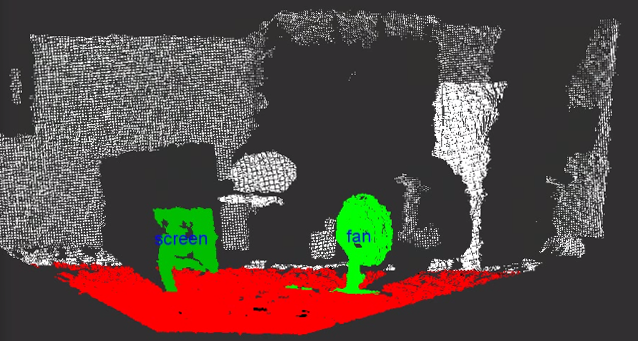
\includegraphics[width=\textwidth]{mono_recon.png}
	\caption{\textbf{reconnaissance mono-vue} - Le résultat de la classification sur les objets segmentés où une écran et un ventilateur étaient reconnus. En rouge le plan du sol et en blanc les points à plus de 3 mètre considérés comme plus bruités. Un remarque pour les ombres infra-rouges qui occultent les objets}
	\label{fig:mono_recon}   
\end{figure}

\section{Localisation et suivi d'objet}

\subsection{Définition de repères}

Se placer dans différents repères permet d'avoir des référentiels plus naturels pour chaque type de composant du robot et pour les objets placés dans la scène. On définit quelques repères et conventions de base pour faciliter la localisation. D'abord le repère de la base du robot est orthonormale positif, où le déplacement vers l'avant correspond à l'axe $\vec{x}$, vers la gauche à l'axe $\vec{y}$ et vers le haut à l'axe $\vec{z}$. Un deuxième référentiel utilisant les mêmes conventions positionne le capteur RGB-D par rapport au robot. Enfin, le dernier référentiel correspond au repère optique du capteur orienté selon la convention usuelle pour les images avec l'axe $\vec{x}$ orienté vers la droite, l'axe $\vec{y}$ vers le bas et enfin l'axe $\vec{z}$ vers l'avant. Ces trois repères permettent d'orienter tous les éléments aperçus par le robot dans l'environnement de façon pratique.

Une méthode de transformation entre repères permet ensuite le passage de l'un à l'autre. On peut ainsi obtenir la position de l'objet  dans le repère global d'après sa détection par la caméra. La transformation entre une base $a$ et une autre $b$ est faite par une matrice de transformation classique, décrit par l'équation \ref{eq:mat_rotation}. 

\begin{equation}
	\mathbf{R}^{a}_{b} = 
	\begin{bmatrix} 
	 	\cos \theta &  -\sin \theta & \Delta x \\ \sin \theta & \cos \theta & \Delta y \\ 0 & 0 & 1
	 \end{bmatrix}
	\label{eq:mat_rotation}
\end{equation}

où $\theta$ équivaut à l'angle entre les deux repères et $\Delta x$ et $\Delta y$ sont les translations linéaires entre eux.

\subsection{Bases mobiles}

\subsubsection{Estimation de l'odométrie}

Certains robots sont dotés de capteurs capables d'estimer de façon
approximative son dépla-cement. C'est aussi le cas du robot utilisé qui
possède des roues codeuses capables d'estimer la rotation angulaire des
roues. Pour le cas d'un robot différentiel, où chaque roue peut être
commandée indépendamment, le déplacement et l'orientation suit les équations suivantes:

\begin{equation}
	\begin{array}{rcl}
		\delta x_t &=& \delta s_t \cdot cos(\theta_{t-1}) \\
		\delta y_t &=& \delta s_t \cdot sin(\theta_{t-1}) \\
		\delta \theta_t &=& \frac{\delta \omega_{g} + \delta \omega_{d}}{d_{r}}\\
		\delta s_t &=& \frac{\delta \omega_{g} + \delta \omega_{d}}{2}						
	\end{array}
\end{equation}
$\omega_g$ et $\omega_d$ sont des respectives variations angulaire des roues et $d_r$ est la distance entre elles. Une intégration, au sens mathématique \ref{eq:integ}, de la différence entre
l'odométrie entre deux intervalles de temps permet de retrouver la position global du robot.

\begin{equation}
	\begin{array}{rcl}
		x_t &=& x_{t-1} + \delta x_{t} \times cos(\theta_{t-1}) - \delta y_{t} \times sin(\theta_{t-1}) \\
		y_t &=& y_{t-1} + \delta x_{t} \times sin(\theta_{t-1}) + \delta y_{t} \times cos(\theta_{t-1}) \\
		\theta_t &=& \theta_{t-1} + \delta\theta_{t}
	\end{array}
	\label{eq:integ}
\end{equation}

\subsection{Filtre de Kalman }

Afin de pouvoir utiliser le déplacement du robot par rapport aux objets pour les identifier, il est d'abord nécessaire de les localiser et les suivre. À cause
de la divergence de l'odométrie, l'imprécision de la segmentation et le calcul
du centroïde de l'objet, la position estimée est fortement bruitée et rend la suivie et identification infaisable
lorsque plusieurs objets sont trop proches. Nous utilisons donc un filtre de Kalman pour corriger cette erreur de mesure et fournir une estimation plus fiable de la position des objets.

Classiquement le filtre de Kalman est mis à jour selon deux étapes : 

\subsubsection{Prédiction} Une première de prédiction qui utilise le modèle linéaire $\textbf{F}_{k}$ pour décrire l'évolution des états au long du temps avec son bruit de process, $\textbf{Q}_{k}$, associé et qui estime \textit{a priori} la covariance de l'erreur $\textbf{P}_{k|k-1}$. Formellement, on utilise les équations \ref{eq:kalman_prediction}

\begin{equation}
	\begin{array}{ccl}
		\hat{\textbf{x}}_{k|k-1} &=& \textbf{F}_{k}\hat{\textbf{x}}_{k-1|k-1} + \textbf{B}_{k} \textbf{u}_{k-1}\\
		\textbf{P}_{k|k-1} &=& \textbf{F}_{k} \textbf{P}_{k-1|k-1} \textbf{F}_{k}^{T} + \textbf{Q}_{k}
	\end{array}
	\label{eq:kalman_prediction}
\end{equation}

\noindent Où les variables sont :\\
$\textbf{F}_{k}$ : la matrice de dynamique du système définie comme identité dans notre cas, si l'on considère que l'objet reste immobile\\
 $\textbf{u}_{k}$ : l'entrée de commande, nulle dans notre cas\\
 $\textbf{B}_{k}$ : la matrice qui relie l'entrée de commande $u$ à l'état $x$, nulle également\\
$\textbf{P}_{k|k-1}$ : la matrice d'estimation a priori de la covariance de l'erreur \\
$\textbf{Q}_{k}$ : la matrice de covariance du bruit de process, diagonale dans notre cas.\\

\noindent Avec: \\
$\textbf{z}_{k}$ \space \space: observation ou mesure du process à l'instant k \\
$\textbf{H}_{k}$ \space : matrice qui relie l'état $\textbf{x}_{k}$ à la mesure$ \textbf{z}_{k}$\\
$\textbf{P}_{k|k}$ : matrice d'estimation a posteriori de la covariance de l'erreur\\
$\textbf{R}_{k}$ \space \space : matrice de covariance du bruit de mesure

\subsubsection{Innovation}
Une deuxième mise à jour, où l'observation est incorporée dans le calcul de l'innovation, $\tilde{\textbf{y}}_{k}$, et du gain de Kalman, $\textbf{K}_{k}$ est décrite par l'équation \ref{eq:innovation}.

\begin{equation}
	\begin{array}{ccl}
		\tilde{\textbf{y}}_{k} &=& \textbf{z}_{k} - \textbf{H}_{k}\hat{\textbf{x}}_{k|k-1} \\
		\textbf{S}_{k} &=& \textbf{H}_{k}\textbf{P}_{k|k-1} \textbf{H}_{k}^{T}+\textbf{R}_{k} \\
		\textbf{K}_{k} &=& \textbf{P}_{k|k-1}\textbf{H}_{k}^{T}\textbf{S}_{k}^{-1} \\
		\hat{\textbf{x}}_{k|k} &=& \hat{\textbf{x}}_{k|k-1} + \textbf{K}_{k}\tilde{\textbf{y}}_{k} \\
		\textbf{P}_{k|k} &=& (I - \textbf{K}_{k} \textbf{H}_{k}) \textbf{P}_{k|k-1}
	\end{array}
	\label{eq:innovation}
\end{equation}
\noindent Avec :\\
 $\textbf{z}_{k}$ : l'observation s'agit de la position de l'objet segmenté dans le repère absolu\\
$\textbf{H}_{k}$ : la matrice qui relie l'état $\textbf{x}_{k}$ à la mesure $ \textbf{z}_{k}$ : Ici, il s'agit d'une matrice identité puisque tout est réalisé dans le repère absolu.\\
$\textbf{P}_{k|k}$ : la matrice d'estimation \textit{a posteriori} de la covariance de l'erreur\\
$\textbf{R}_{k}$ : la matrice de covariance du bruit de mesure. Matrice diagonale dans notre cas.

\subsubsection{Suivi multi-cibles}
Le caractère monomodal du filtre de Kalman nous contraint à ne pouvoir suivre qu'un seul objet à la fois. Pour obtenir un suivi multimodal, il faut que plusieurs filtres tournent en parallèle. Ainsi, le problème passe d’estimer la position d'un seul objet à celui de décider quelle observation appartient à quel filtre. Pour ce faire, nous définissions une matrice de distances entre chaque nouvelle observation et les états courants de chaque filtre de Kalman déjà créé.
Ensuite, les nouvelles observations sont utilisées pour mettre à jour les filtres de Kalman dont l'estimation est la plus proche selon cette matrice. Avant toute mise à jour, on vérifie que la distance entre l'observation et l'estimation du filtre ne dépasse pas un certain seuil. Pour chaque observation qui n'a pas pu être associée à un filtre déjà existant, on crée alors un nouveau filtre.

\section {Reconnaissance Multi-vue}

\subsection {Chaînes de Markov Cachées}

Le déplacement physique du robot produit une séquence
d'observations, sous différents points de vues, d'un même objet. On exploite
l'information odométrique entre les différentes vues pour renforcer l'estimation de la vue d'un objet. De cette manière, l'évolution de la
reconnaissance au cours du temps est représentée par un processus
stochastique, dont une modélisation possible consiste à le traiter
de façon discrète dans un espace d'état. Ayant l'apriori que la
dernière image et le dernier déplacement suffisent pour faire cette
prédiction (c'est-à-dire en respectant la propriété de Markov de premier
ordre), le processus stochastique est modélisée par une
chaîne de Markov cachée.

Concrètement, les états cachés correspondent à des vues d'objets connus au
préalable et déjà stockés dans la mémoire du robot. Cela contraint le
nombre d'états et garantie que la chaîne soit finie. Puis, une
matrice de transition, $a_{i,j}$, décrit l'évolution du processus. C'est cette matrice de transition qui permet de prendre en compte l'odométrie et la transition entre les vues d'un même objets. Enfin, une autre matrice, $\mathrm{P}\big( y_1 \ | \ k \big)$, dite matrice d'émission, estime la vraisemblance entre l'observation
et les états de la chaîne.

Plus précisément,  $a_{i,j}$ est définie en fonction de l'angle $\delta_{angle}$, calculé par \ref{eq:delta_ang} qu'a parcouru le robot par rapport à l'objet entre deux vues successives. Dans notre modèle, on considère que $a_{i,j}$ est nulle si $i$ et $j$ sont deux vues d'objets différents. Pour deux vues $i$ et $j$ d'un même objet, séparées d'une distance $d$, le poids accordé à $a_{i,j}$ sera d'autant plus fort que $\delta_{angle}$ et $d$ sont proches. D'autre part, la matrice d'émission $\mathrm{P}\big( y_1 \ | \ k \big)$ correspond à la similarité entre l'histogramme d'un objet segmenté $y$ et celui d'une vue d'objet dans la base de données $k$, normalisés par l'équation \ref{eq:dist_norm}. La similarité est calculée comme l'inverse de la distance Chi square définie à la section \ref{sec:rec_mono}.
  \begin{equation}
  \begin{array}{rcl}
    \vec{d}_0 &=& p_0 - p_{obj}\\
    \vec{d}_1 &=& p_1 - p_{obj} \\
     \delta_{angle} &=& atan(\vec{d}_1) - atan(\vec{d}_0)
  \end{array}
  \label{eq:delta_ang}
  \end{equation}
La transformation des distances des histogrammes en probabilité est faite d'après la normalisation suivant :
\begin{equation}
	\mathbb{P}(y|x, database) = \frac{\sum_a d_a^x - d_y^x}{\sum_b \sum_c d_c^x - d_b^x}
	\label{eq:dist_norm}
\end{equation}
où $x$ est l'image de teste et y un élément de la base de donné. Dans le cas du plus proches voisin la normalisation prend en compte seulement les k plus proches histogrammes, en contraste au approche \textit{bruta force}.

Une autre modélisation possible aurait été d'avoir une chaîne de Markov
cachée distincte pour chaque objet et ensuite décider à chaque pas de temps le
processus le plus vraisemblable. Cette modélisation peut être vue comme un sous-ensemble du cas
précédent où les transitions entre deux objets ne sont pas
considérées. Pourtant, il peut arriver que deux objets soit considérés comme positionnés au même endroits, ou bien que des objets mobiles fusionnent (par exemple, une personne qui viendrait s'asseoir sur une chaise, ou encore un personne
qui commence à marcher) \footnote{Le fait de se mettre en mouvement
  altère les formes d'une personne, ce qui rend possible sa détection
  comme un nouvel objet.}.

\subsection{Algorithme de Viterbi}

Reste donc à extraire des informations de la modélisation Markovienne proposée.
La séquence d'états la plus vraisemblable qui pourrait avoir géneré
les observations  $y_1,\dots, y_T$, correspond normalement à la séquence d'objets reconnus.
Afin de retrouver cette séquence, aussi appellée chemin, on fait 
appel à la programmation dynamique, et plus spécifiquement à l'algorithme de Viterbi, d'où le nom chemin de Viterbi.
L'algorithme retrouve de façon récursive l'état courant le plus probable, en
prenant en compte seulement les observations jusqu'à un instant donné et son
estimation aux instants antérieurs. Ceci se traduit par les équations \ref{eq:viterbi}

\begin{equation}
  \begin{array}{rcl}
    V_{1,k} &=& \mathrm{P}\big( y_1 \ | \ k \big) \cdot \pi_k \\
    V_{t,k} &=& \max_{x \in S} \left(  \mathrm{P}\big( y_t \ | \ k \big) \cdot a_{x,k} \cdot V_{t-1,x}\right)
  \end{array}
	\label{eq:viterbi}
\end{equation}

Ici, $V_{t,k}$ représente la probabilité que la séquence d'états la plus probable finisse dans l'état $k$, ayant généré les observation à l'instant $t$, tandis que $\pi_i$ représente la probabilité initiale de se retrouver en chaque état. Pour retrouver le chemin de Viterbi, il suffit de trouver le maximum de $V_{t,k}$ :

\begin{equation}
  \begin{array}{rcl}
    x_T &=& \arg\max_{x \in S} (V_{T,x})
  \end{array}
\end{equation}

\subsection {Graphe d'aspect polaire}
%\celine{Je trouve que cette section n'est pas très utile en fait. Tu fais référence ailleurs à un graphe d'aspect (je ne sais plus où). Si tu veux, tu peux mettre cette partie dans les annexes et y faire référence à l'endroit du rapport ou tu en parles}

On considère que les objets sont décrits par deux dimensions
d'information : une spatiale, représentant la position absolue de l'objet
dans l'environnement ainsi que les positions relatives où l'objet a été
visualisé, et une autre dimension visuelle, donnée par les descripteurs
géométriques, de couleurs et de texture. On cherche à représenter cette description dans un référentiel unique. Le graphe d'aspect permet de coupler
l'ensemble des images suivant ses possibles transitions spatiales, ce qui
résulte dans la possibilité de construire le modèle à la volée et de
jouer avec sa densité d'information - le nombre d'images intégrées au modèle.

\begin{figure}[H]
  \centering
  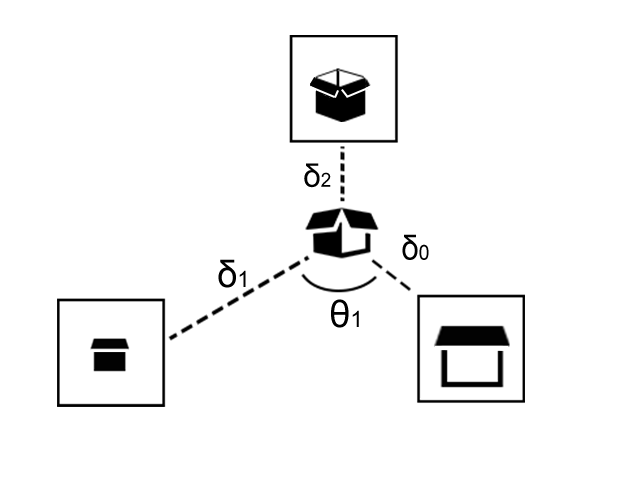
\includegraphics[width=0.4\textwidth]{object_model.png}
  \caption{Représentation des objets par un modèle polaire}
	\label{fig:graphe_polaire}
\end{figure}

Un référentiel polaire entrelace toutes ces informations
de façon à représenter la position spatiale d'où l'observation a été
faite, comme représenté dans l'image \ref{fig:graphe_polaire}. Pour la
construction du modèle les conventions suivantes ont été adoptées :
\begin{itemize}
\item l'angle zéro est attribué à la première observation
\item L'origine du référentiel est la position globale de l’objet
\item Les features sont labellisées d'après le déplacement angulaire
  et la distance au centroïde de l'objet.
\end{itemize}

Une grande majorité des features visuelles ne sont pas invariantes à l'échelle, et ce d'autant plus si la résolution de l’image joue un rôle critique pour la
détection de features, comme les patches SIFTs. Ainsi, prendre également en compte la distance à laquelle l’image a été prise peut être intéressant pour limiter la
classification à une échelle valable.